% !TEX encoding = UTF-8 Unicode
\documentclass{article}

\usepackage{polski}
\usepackage[utf8]{inputenc}
\usepackage{subfig}
\usepackage{graphicx}

\usepackage[a4paper, left=2.5cm, right=2.5cm, top=3.5cm, bottom=3.5cm, headsep=1.2cm]{geometry}

\linespread{1.3}

\begin{document}
	
	\begin{titlepage}
		\centering
		{\scshape\LARGE Politechnika Wrocławska \par}
		{\scshape\Large Katedra Informatyki Technicznej\par}
		
		\vspace{1.5cm}
		{\scshape\Huge Bazy Danych \par}
		\vspace{1.5cm}
		
		\vspace{2cm}
		{\Large\itshape Magdalena Biernat\par}
		{\Large\itshape Mateusz Bortkiewicz\par}
		\vfill\flushleft\large
		
		\normalsize	\centering	\vspace{3cm}
		Prowadzący\par
		dr inż. Tomasz Janiczek 
		
		\vfill
		{\large \today\par}
	\end{titlepage}
	\newpage
	\section{Opis "świata rzeczywistego"}
	Opis "świata rzeczywistego" - aplikacja "Domowa wypożyczalnia wideo"
	\subsection{Opis zasobów ludzkich}
		- Głowa rodziny, tudzież osoba wyznaczona w domu administruje i zarządza aplikacją desktopową "Domowa wypożyczalnia wideo". Może ona usuwać i dodawać użytkowników, resetować hasła, zwracać/wypożyczać administracyjnie egzemplarze filmów, usuwać tytuły filmów, wycofywać z użycia egzemplarze filmów, a także wykonywać to co zwykły użytkownik
		- Użytkownik, mieszkaniec domostwa może dodać lub edytować tytuły filmów oraz egzemplarze do tytułów obecnych już filmów. Może wypożyczać dostępny egzemplarz filmu
		- Wypozyczenie posiada identyfikator domownika, identyfikator egzemplarza filmu a także datę wypożyczenia i informację czy film jest zwrócony.
		- Użytkownik może edytować swoje konto, tj. zmieniać hasło.
	\subsection{Przepisy}
		Liczba wypożyczonych jednocześnie egzemplarzy przez danego użytkownika nie może być większa niż trzy. Nie istnieje termin zwrotu - wypożyczenie jest bezterminowe. Nieaktywny użytkownik nie może się zalogować na konto i wypożyczyć/zwrócić filmu.
	\subsection{Dane techniczne}
		 Obsługa konta, bazy wideo i wypożyczeń powinna być dostępna przez aplikację desktopową połączoną z bazą danych.
		Wypożyczający loguje się do konta za pomocą loginu i hasła. Hasło nie jest przechowywane w bazie danych (jest to jedynie zahaszowane hasło)
	
	\section{Wymagania funkcjonalne i niefunkcjonale}
	\subsection{Wymagania funkcjonalne}
	\begin{itemize}
	\item aplikacja ma mieć możliwość wyszukiwania\$dodawania\$edytowania\$usuwania filmów do bazy danych
	\begin{itemize}
		\item wyszukiwać i dodawać filmy może każdy użytkownik
		\item usuwać i edytować może tylko administrator systemu
	\end{itemize}
	\item aplikacja ma mieć możliwość edytowania danych użytkownika
	\item  dodawać nowego użytkownika może tylko administrator
	\item aplikacja ma mieć możliwość wyszukiwania\$dodawania\$edytowania\$usuwania tytułów filmów do bazy danych 
	\begin{itemize}
		\item wyszukiwać i dodawać tytuły może każdy użytkownik
		\item usuwać i edytować może tylko administrator systemu
	\end{itemize}
	\item obsadę może dodawać każdy użytkownik
	\item aplikacja pokazuje wypożyczone pozycje i listę życzeń (filmy, których egzemplarze nie są umieszczone w bazie danych)
	\end{itemize}
	\subsection{Wymagania niefunkcjonalne}	
	\begin{itemize}
		\item ilość domowników nie wpływa na szybkość działania systemu
		\item ilość filmów/tytułów/użytkowników etc. Jest ograniczona tylko pojemnością dysku na którym stoi baza danych
		\item przyjazny interfejs użytkownika
		\item liczba błędów w aplikacji przez pierwszy miesiąc od wydania aplikacji nie może przekroczyć 5		
	\end{itemize}
\newpage
	\section{Diagram przypadków użycia}
	\begin{figure}[!ht]	
		\centering
		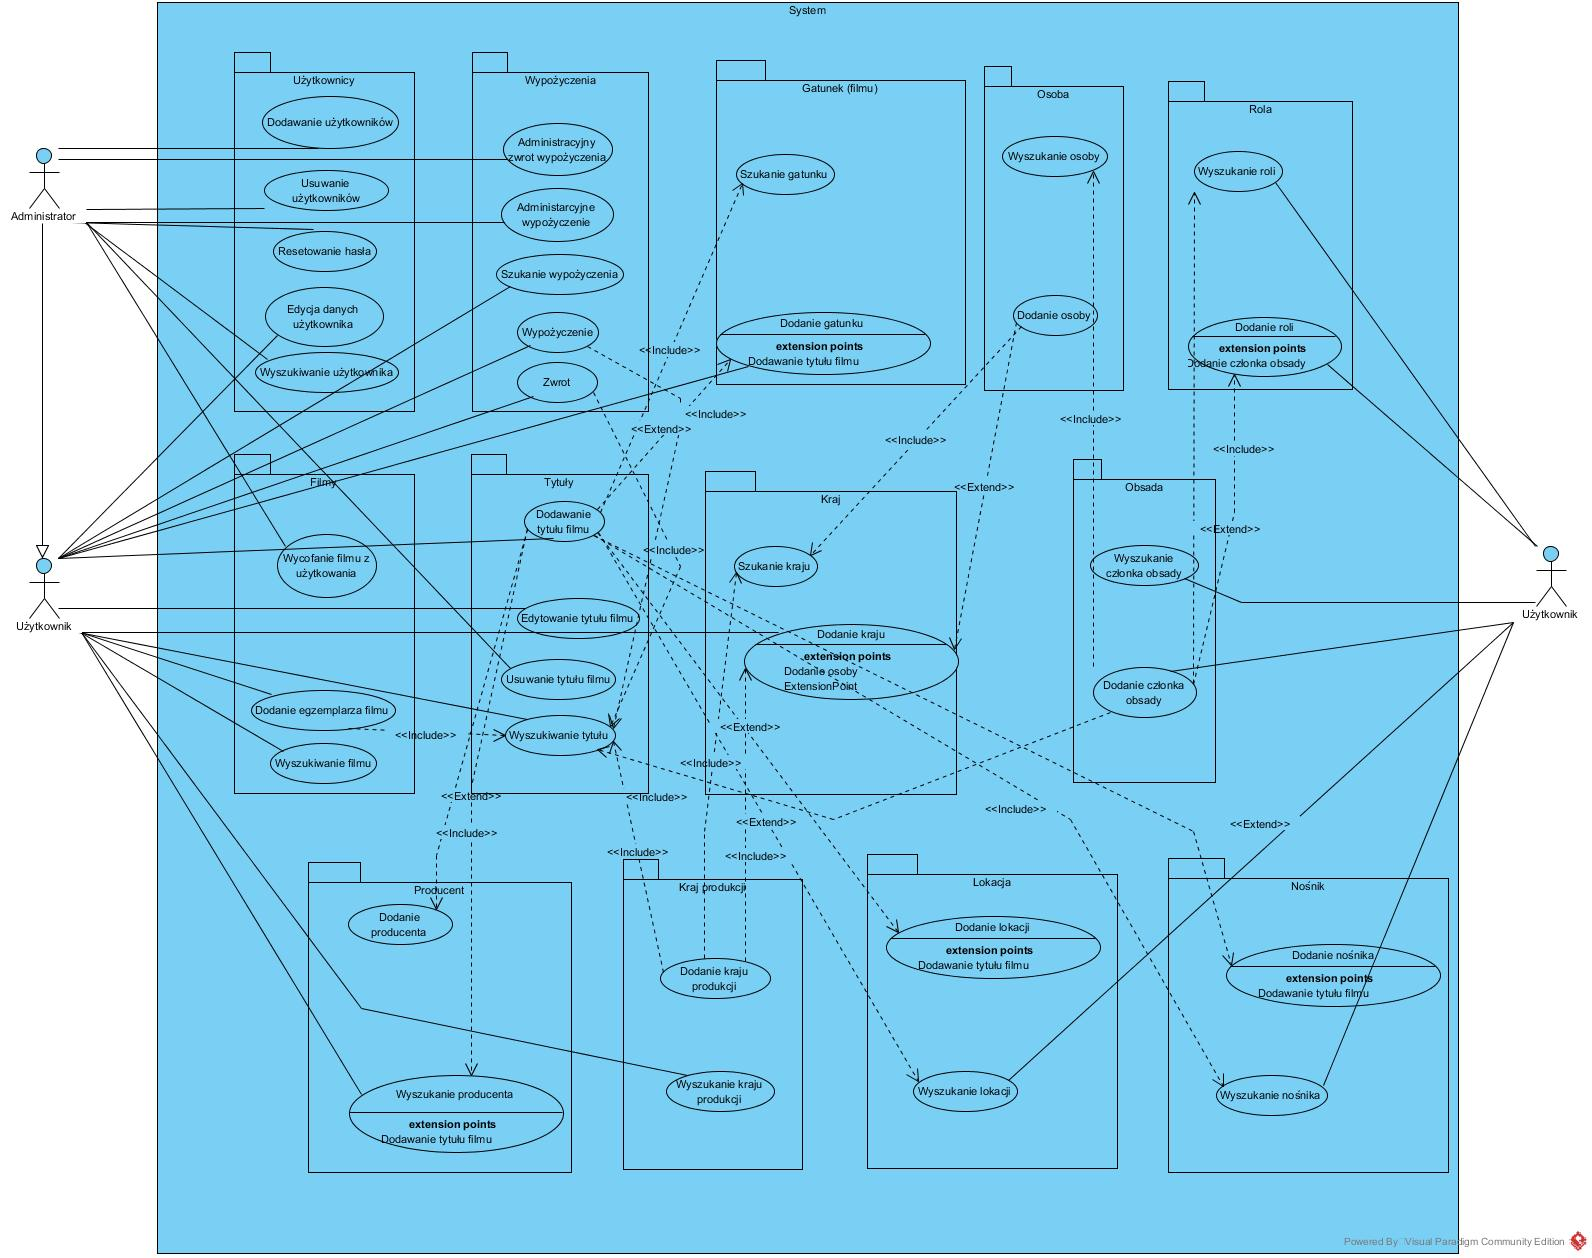
\includegraphics[height=13cm]{PU.jpg}
		\caption{Diagram PU}
		\label{fig:obrazek 1}
	\end{figure}
\newpage
	\section{Diagram związków encji}
		\begin{figure}[!ht]	
		\centering
		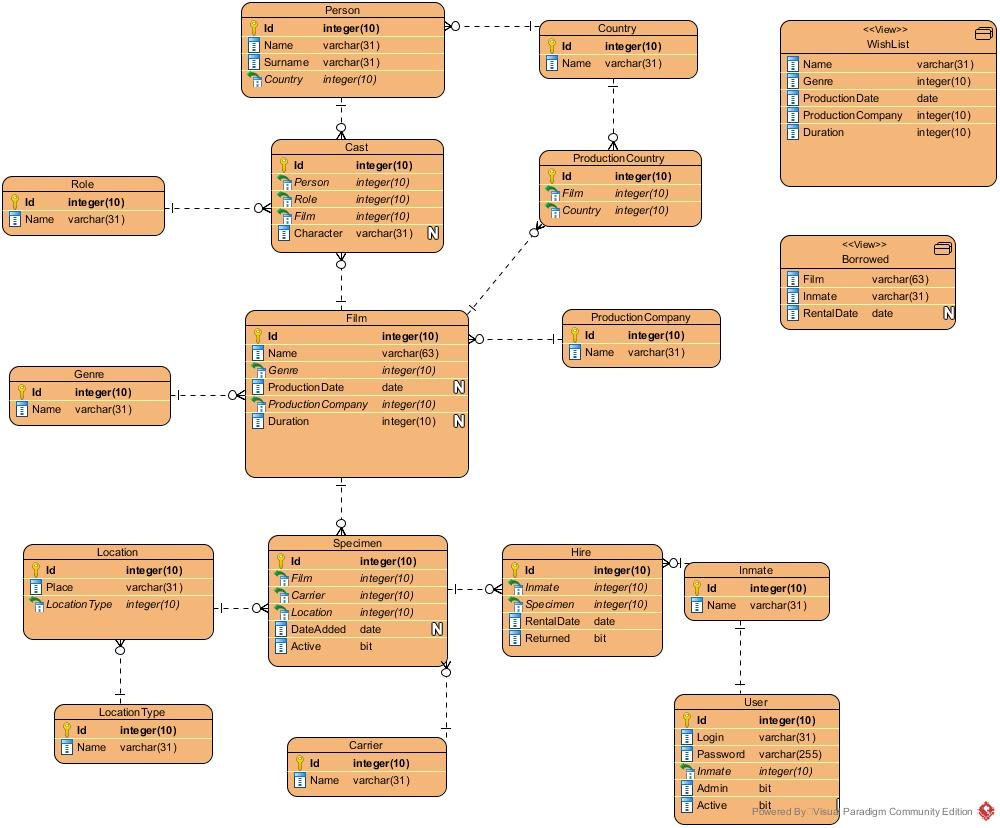
\includegraphics[height=14cm]{diagram_zwiazkow_encji.jpg}
		\caption{Diagram związków encji}
		\label{fig:obrazek 2}
	\end{figure}
\end{document}